\newcommand\version{v1}
\problemname{Friends}
$N$ friends are playing a game. The game is played on a row of $L$ squares, numbered from $0$ to $L - 1$, where squares $i$ and $i+1$ are adjacent to each other. At most one friend stand on each square
at any given time. In each step of the game, one friend jumps from its current square to a new (non-occupied) square.

In any moment of the game, the \emph{score} of a friend is the length of the longest contiguous segment
of friends it is part of. This means that if a friend stands on some position $x$, and there are friends
on positions $a, a + 1, ..., x - 1, x, x + 1, ..., b - 1, b$, the score of the friend is $b - a + 1$.

The total score of the game is the sum of scores for all friends. At various times during the game, the friends wonder what their current total score is.

\section*{Example}
Assume that we have $N = 3$ friends playing on a strip of length $L = 7$. Initially,
their locations are $1, 3, 4$. The score of the friend on location 1 is just 1, since it has no friends
to the left or to the right. However, the friends at locations 3 and 4 make a segment of length 2, so
each of their scores are 2. The score of the game is thus $1 + 2 + 2 = 5$.

The first jump is from position $4$ to $2$, making the new positions $1, 2, 3$. Here, all friends
make up a segment of length 3, so each of the friends have score 3, making the total score 9.

The second and final jump is from $3$ to $0$, resulting in the positions $0, 1, 2$. All friends
still make up a segment of length 3, so the score is unchanged from last time, i.e. it is still 9.

\begin{figure}[h!]
  \centering
  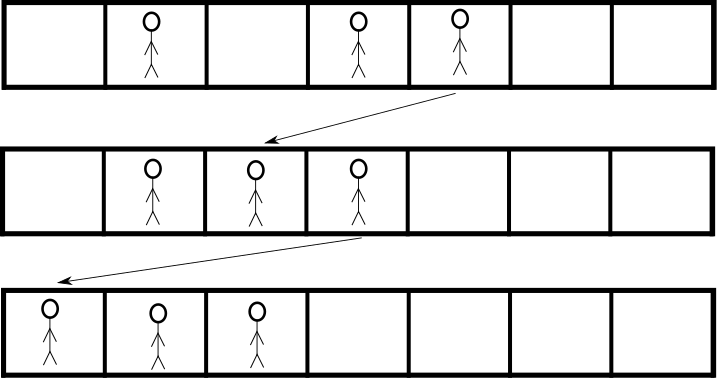
\includegraphics[width=0.8\textwidth]{sample.png}
  \caption{Illustration of the example}
\end{figure}

\section*{Task}
You will get all the jumps in the game, one by one. At some points, the friends will ask what the current score is. Your task is to
implement the functions \texttt{init(N, L, P)}, \texttt{jump(A, B)}, and \texttt{score()}:
\begin{itemize}
  \item \texttt{init(N, L, P)} - this function will be called exactly once by the judge, at the start of the game.
  \begin{itemize}
    \item \texttt{N}: the number of friends playing.
    \item \texttt{L}: the number of locations the game is being played on.
    \item \texttt{P}: an array with $N$ elements. \texttt{P[i]} ($0 \le i < N$) contains the original position of the $i$:th friend.
    \item The function has no return value.
  \end{itemize}

  \item \texttt{jump(A, B)} - this function will be called once for every jump, in the order they are made.
  \begin{itemize}
    \item \texttt{A}: the position a friend is jumping from ($0 \le A < L$). This position will always contain a friend at the time of the jump.
    \item \texttt{B}: the position a friend is jumping to ($0 \le B < L$). This position will never contain a friend at the time of the jump.
    \item The function has no return value.
  \end{itemize}

  \item \texttt{score()} - this function will be called when the friends wish to know their current scure.
  \begin{itemize}
    \item The function should return the current score in the game.
  \end{itemize}

\end{itemize}

\section*{Subtasks}
The problem consists of a number of subtasks. Each subtask gives some amount of points, and to pass
the subtask you must pass all the test cases in the subtask.

Let $J$ be the number of calls to \texttt{jump} and $S$ the number of calls to \texttt{score}.

\begin{tabular}{|l|l|l|}
  \hline
  \textbf{Subtask} & \textbf{Points} & \textbf{Limits} \\ \hline
  1 & 9 & $1 \le N, L \le 1\,000$,  $S + J \le 2\,000$ \\ \hline
  2 & 17 & $1 \le N, L \le 100\,000$, $J = 0$, $S = 1$ \\ \hline
  3 & 14 & $1 \le N \le 100\,000$, $1 \le N \le 10^9$, $J = 0$, $S = 1$ \\ \hline
  4 & 38 & $1 \le N, L \le 100\,000$, $S + J \le 200\,000$ \\ \hline
  5 & 22 & $1 \le N \le 100\,000$, $1 \le N \le 10^9$, $S + J \le 200\,000$ \\ \hline
\end{tabular}

\section*{Input format}
The sample judge reads input in the following format:

\begin{itemize}
  \item line $1$: \texttt{N L Q}
  \item line $2$: \texttt{P[0] P[1] .. P[N - 1]}
  \item lines $3$ to $3 + Q - 1$: each line represents either a jump or a score question.
    If the line is \texttt{0 A B}, a jump from $A$ to $B$ is to be made, and if the line is \texttt{1} a scoring question is to be made.
\end{itemize}

\section*{Output format}
For each scoring question, the judge writes a line with the return value of \texttt{score()}.
